\section{Implementation Details}
\label{sec:implementation}

In this section we will briefly describe our implementation of the algorithms described in the above sections. In particular, we highlight optimizations made and provide results suggesting that our algorithms can feasibly scale to industrial-sized applications.

\subsection{Enabling Technology and Prototype}

In previous work we have reported on the usage of Prolog as a means to build a
proof-of-concept prototype for our technique~\cite{Lucio:10}. The experiments
performed using Prolog were inconclusive regarding the scalability of our
technique given that the path condition construction algorithm as now described in \cref{sec:building_pcs} lacked a formal understanding, as well as several other
imprecisions. As such, no performance optimisations were attempted.

Through our sponsorship by the NECSIS (Network for the Engineering of Complex
Software-Intensive Systems for Automotive Systems) project, we have the
opportunity to apply our verification technique in an industrial setting. In
order to achieve high performance in this setting, despite the complexities of
verification techniques, we were required to choose an underlying efficient
implementation framework. Our goals were to select a framework which: 1) allows
graph manipulation natively. This detaches us from the worries of building and
optimising our own subgraph isomorphism NP-complete algorithms, which are
constantly used during path condition construction; and 2) allows detailed control over
graph manipulation such that the implementation of complex optimizations is feasible. These optimizations are potentially required to apply our technique to large and complex model transformations.

We have chosen T-Core~\cite{DBLP:journals/eceasst/SyrianiV10,SyrianiVanghel:13}
as our graph manipulation framework.
Aside from satisfying our basic requirements described above, T-Core allows
for native rewriting of typed graphs, which considerably eases our implementation
effort. The algorithms described throughout this work have been implemented by scheduling T-Core
graph manipulation primitives using the Python programming language. 

\subsection{Complexity}
\label{sec:complexity}

Let us motivate our discussions of optimisation and performance by providing an
approximate formula for the complexity of the path condition construction and
property proof algorithms presented in Sections~\ref{sec:building_pcs}
and~\ref{sec:verif_dsltrans_props}.

\subsubsection{Path Condition Generation}
Recall that a DSLTrans transformation is composed of rules arranged in layers.
The path condition generation algorithm described in \cref{sec:building_pcs}
moves through these layers and combines rules into viable path conditions.

Let the number of rules in the transformation be $r$.  Then, the maximum number
of path conditions that can be created is $2^{r}$. Each path condition will
either represent a rule or not, and therefore the $2^{r}$ path conditions
represent all possible rule combinations. Note that this case assumes that all
path conditions are viable. In practice, unsatisfied rule dependencies will
prevent some rule combinations, reducing the number of path conditions created.

As discussed in \cref{sec:building_pcs}, the path condition generation algorithm builds these path conditions by
considering all possibilities of how a rule can combine with a path condition. This
combination step is composed of two algorithmic components. The first is to
determine all positions where the rule matches over the path condition. Let this
matching step be $m$. Note that this matching step is dependent on the size of the rules.

The second step of the combination step is to "glue" the rule at all matching
positions. Let this step be termed $g$. This step is linear in the size of the rule to be glued multiplied by the number of times the rule has matched in step $m$.

Note that $m$ and $g$ could be quite expensive operations. However, in
our implementation, these steps are implemented using the efficient T-Core graph
manipulation framework.

\begin{equation}
\label{eq:complexity}
\mathcal{O}\big({2^r \cdot (m + g)}\big)
\end{equation}

\cref{eq:complexity} presents the time and space complexity for the path condition generation algorithm.

\subsubsection{Property Proof}
\label{subsubsec:complex_prop_proof}
For our property proving algorithm, recall that each path condition created is examined to see if the property in question holds.

As mentioned in \cref{sec:verif_dsltrans_props}, a path condition must be \\matched by the property. However, different elements in the path condition may overlap (have been matched on) on the same elements in the input model, as described in \cref{sec:prop_satisfaction}.
Therefore, an operational step is required to resolve this ambiguity. One solution is to produce all possible path conditions, where for each pair of overlapping elements in a path condition, one new path condition is produced where they are merged, and one new path condition where they are not.

The complexity of this ``disambiguation step'' will be proportional to the average number of overlapping elements in the path condition, and will be denoted by the term $d$ in this discussion. Practically, $d$ will be dependent on how rules are combined during the path condition generation algorithm. Future work will precisely detail how the characteristics of the transformation affect the algorithm's complexity.

The complexity of the matching step will then be linear in the size of the set of path conditions. The property matching step itself ($p$) will then be linear in the size of the property and path conditions. Again, in practice $p$ is implemented using the T-Core framework.

\begin{equation}
\label{eq:complexity2}
\mathcal{O}\big({2^r \cdot 2^d \cdot p}\big)
\end{equation}

\cref{eq:complexity2} shows time and space complexity for the property proving step.

\subsection{Optimisations}
\label{sec:optimization}

In order to tackle the time and space complexities of the path condition
construction and property proof algorithms we have employed several engineering 
strategies. In the following paragraphs we describe the most relevant of these
strategies.

\begin{itemize}
\item Path condition construction and property proof are very repetitive
processes since most individual rules are often composed and searched in 
the same manner. Since many similar situations have to be investigated during
path condition construction and property proof, memoisation was used whenever
possible to avoid isomorphic graph matching and rewrite operations.
As such caching is heavily used in both algorithms;

\item In \cref{subsubsec:complex_prop_proof} we detail how the overlap of elements in a path condition can be operationally handled by producing two new path conditions for each pair of overlapping elements. Given this procedure is recursive and presents exponential
time complexity, we have performed this ``disambiguation'' step only when strictly necessary:  when performing
property verification on a path condition that contains the elements in
the property.
Note that the fact that  disambiguation is performed in this lazy fashion
allows us to operationally keep path conditions as sets of individual rules.
This makes it possible to heavily reuse pointers to the original transformation
rules when building path conditions, thus reducing the algorithm's space complexity when compared to the explicit representation of
each generated path condition. This also means that, practically,
path condition disambiguation is mostly done on demand during property proving;

\item For property proof we have implemented a strategy to avoid checking path
conditions where the property is sure to hold. The strategy is based on the fact
that if a path condition $B$ contains the same elements as a path condition
$A$ where the property has already been checked successfully, and no additional
elements of the property exist in $B$, then the property also holds
for $B$.
\end{itemize}



\section{Experiments}
\label{sec:experiments}

This section will detail the experiments we performed in order to measure the performance of our technique. We present timing results for two experiments. The first is to obtain timing results for proving two properties on a synthetic transformation, while the second experiment is sourced from our industrial partners.

\subsection{Experimental Setup and Results}

The complexity of \cref{eq:complexity} and \cref{eq:complexity2} suggest that our property proving
approach is intractable in the general case. However, we have provided in \cref{sec:optimization} a number
of concrete optimisations to allow us to prove properties on transformations of
non-trivial size. This section will detail our experiments to determine the
effect of the number of rules in the transformation on the performance of our
implementation.

For our experiment we have used the Police Station transformation as described
in \cref{sec:dsltrans} as a sample transformation. However, in order to
determine the performance characteristics of our approach, we have replicated
the rules within the transformation.

This was achieved by synthetically augmenting the original metamodels by
replicating their elements twice, thus building source and
target metamodels that are three times larger. For example, in the source
metamodel we will now have \emph{Station1} (renamed from the original
\emph{Station} class) and its replicas \emph{Station2} and \emph{Station3}.
These three metamodel elements are distinct from each other and are formally
three different types. We have also added new rules that utilise these new
types, as seen in \cref{fig:replicated_police_station_trafo}.

\begin{figure}[bht] \centering 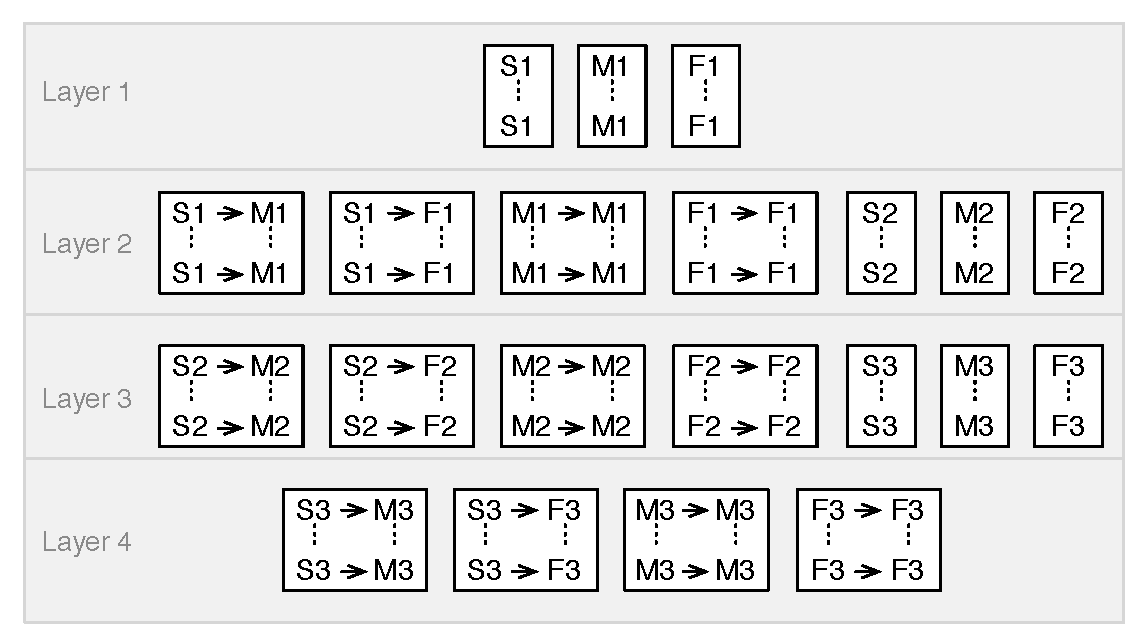
\includegraphics[width=0.48\textwidth]{./figures/policestation_dsltrans/3runtransformation.pdf}
	\caption{Replicated Police Station transformation for performance tests}
	\label{fig:replicated_police_station_trafo}
\end{figure}

Note that for clarity reasons in
\cref{fig:replicated_police_station_trafo} we have abbreviated the element
names \emph{Station}, \emph{Male} and \emph{Female} to \emph{S}, \emph{M} and
\emph{F} respectively. Additionally, the numerical suffix denotes which
replicated metamodel element is represented, as described above.



\renewcommand{\baselinestretch}{1.0}

\subsubsection{Results}

\begin{table*}[htb]
\label{table:results}
\centering
\begin{tabular}{|c|r|r|r|r|r|}
\hline
\rowcolor{Gray}
\parbox[t]{0.04\textwidth}{\# of rules\\} & 
\parbox[t]{0.13\textwidth}{\# of path conds. created\\} 
& \parbox[t]{0.15\textwidth}{Path conds. build time (s)\\}
& \parbox[t]{0.11\textwidth}{Memory used (KB)\\}  
& \parbox[t]{0.18\textwidth}{Proof time for property that holds (s)\\} 
& \parbox[t]{0.20\textwidth}{Proof time for property that does not hold (s)\\}\\
\hline
3	&	8		&	$<$0.01		&	0.08	&	-		&	-		\\
5	&	16		&	0.13		&	0.09	&	0.19		&	0.003	\\
7	&	34		&	0.39		&	0.17	&	1.26		&	0.003	\\
10	&	272		&	1.87		&	1.24	&	2.40		&	0.003	\\
12	&	442		&	2.68		&	1.83	&	3.40		&	0.003	\\
14	&	1156	&	9.00		&	4.98	&	8.38		&	0.003	\\
17	&	9248	&	59.08		&	38.01	&	73.51	&	0.003	\\
19	&	15028	&	97.52		&	60.10	&	140.77	&	0.003	\\
21	&	39304	&	369.19		&	156.79	&	412.02	&	0.003	\\
\hline
\end{tabular}
\caption{Results for creating the set of all path conditions and proving two properties}
\label{tab:scalability_results}
\end{table*}

\reviewer{Table 1, even if it was not experimented to exceed 0.003 seconds when proving for property that does not hold, maybe it would be possible to estimate the maximum time based on that measurement and the complexity formula.}

The results in \cref{tab:scalability_results} were obtained by verifying
the properties in Figures~\ref{fig:dsltrans_prop1}
and~\ref{fig:dsltrans_prop2} on the transformation seen in
\cref{fig:replicated_police_station_trafo}. The experimental platform was
a 2.2 GHz Intel Core i7 machine with 8GB of DDR3 memory running Ubuntu 11.10 and
Python 2.7. For each measurement involving time, we repeated the given
experiment three times and calculated the final result as the average of the
three experiment results. The code used to run our experiments can be found
at~\cite{DSLTransVerif:13}.




\subsubsection{Time Required to Produce Path Conditions}

An important metric for our work is measuring how long it takes to produce the final set of path conditions from a DSLTrans transformation. As seen in \cref{sec:complexity}, this metric depends on the composition of the rules in the transformation's layers.

The first column of \cref{tab:scalability_results} shows the number of
rules for each part of the experiment. In order to provide greater granularity in the data, and determine the precise effect of adding more rules to a layer versus adding another layer of rules, we examine subsets of rules taken from \cref{fig:replicated_police_station_trafo}. For example, the subset with five rules contains the three first rules of layer 1 plus the two first rules of layer 2; the subset with seven rules contains the first three rules of layer 1 plus the four first rules of layer 2; and so on.

\begin{figure*}[htb]
        \centering
        \begin{subfigure}[b]{0.26\textwidth}
                \centering
                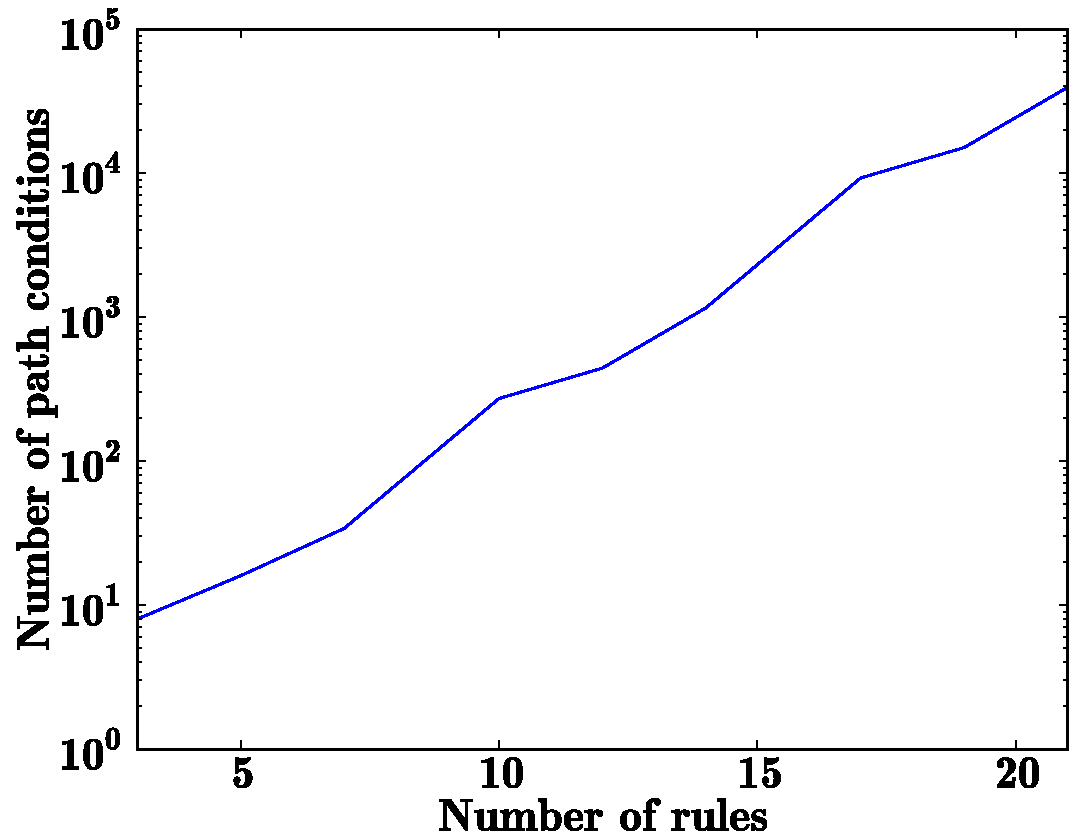
\includegraphics[width=1\textwidth]{./figures/results/rules_vs_pcs.pdf}
                \caption{Number of rules vs. \\path conds. created}
                \label{fig:rules_vs_pcs}
        \end{subfigure}%
        ~~
        \begin{subfigure}[b]{0.26\textwidth}
                \centering
                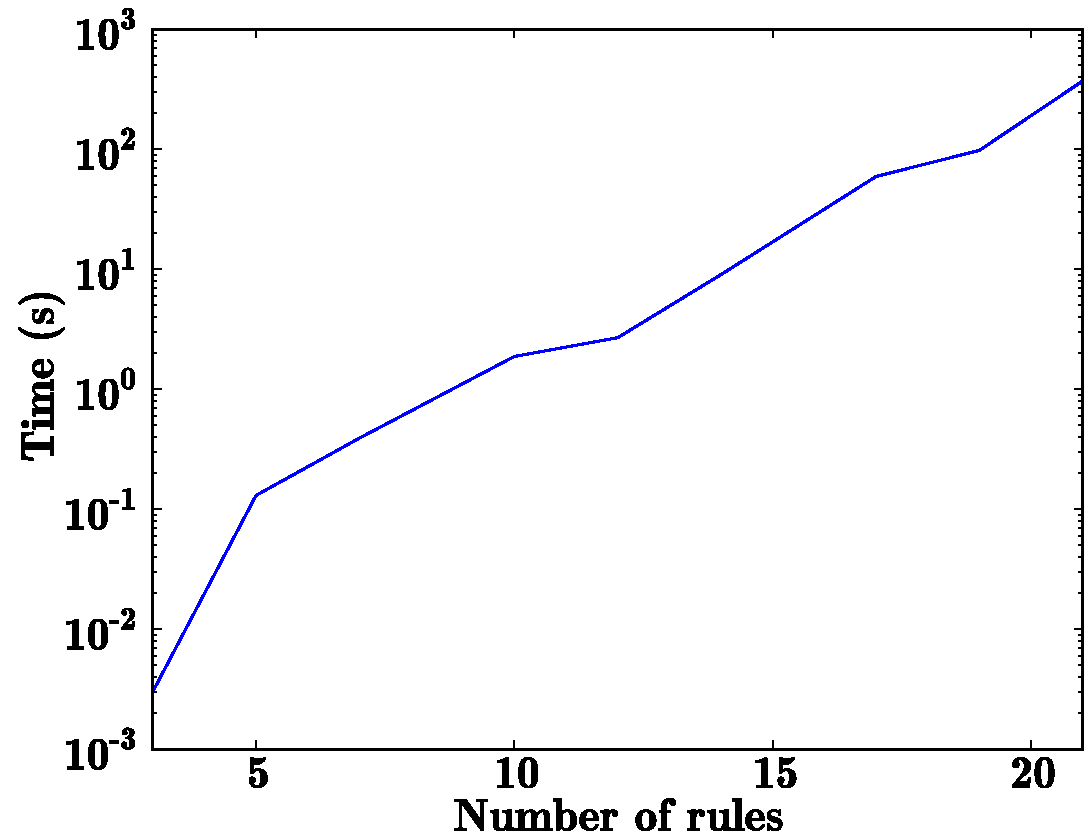
\includegraphics[width=1\textwidth]{./figures/results/rules_vs_time.pdf}
                \caption{Number of rules vs. \\time taken}
                \label{fig:rules_vs_time}
        \end{subfigure}%
        ~~
        \begin{subfigure}[b]{0.26\textwidth}
                \centering
                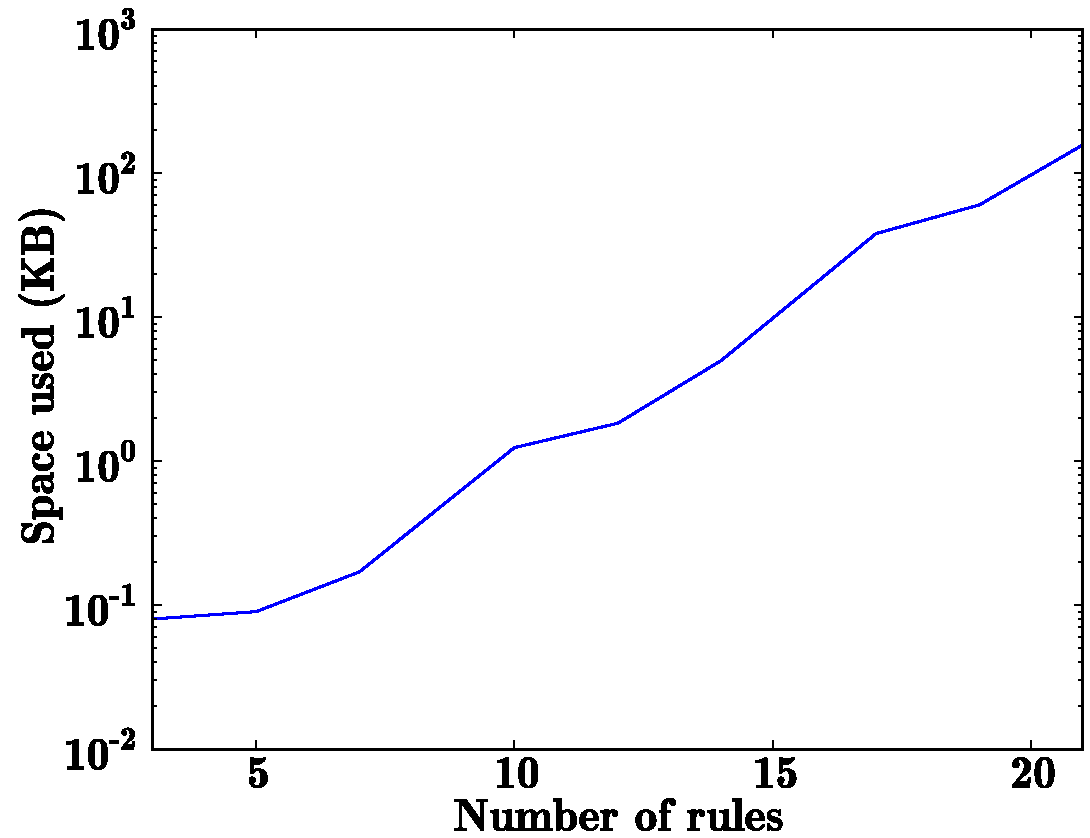
\includegraphics[width=1\textwidth]{./figures/results/rules_vs_memory.pdf}
                \caption{Number of rules vs. \\memory used}
                \label{fig:rules_vs_memory}
        \end{subfigure}%

        \caption{Metrics for the path condition creation process}
        \label{fig:path_condition_building}
\end{figure*}



\cref{fig:rules_vs_pcs} presents the number of path conditions created for
a given number of rules, while \cref{fig:rules_vs_time} graphs the time
taken to create all the path conditions. Both the number of path conditions and
the time required to build them rise steeply with the number of rules, but it
is quite feasible to build path conditions and prove properties for up to 21
rules. As shown later in the section on industrial experimentation, 21 rules
exceeds the number of rules in our industrial case study. It also exceeds the
number of rules in several useful DSLTrans
transformations~\cite{febavava:10,dsltrans_manual,zhang:ACP_APN:11}.

\cref{tab:scalability_results} and \cref{fig:rules_vs_memory} demonstrate that memory consumption is very modest, remaining well under a megabyte for thousands of path conditions. This is due to the optimisations that we perform, such as only storing pointers to path conditions. We are encouraged that this algorithm can scale extremely well in terms of respecting memory constraints.


\subsubsection{Time Required to Prove Properties}

We now examine the time it takes to prove two properties on the transformation based on the number of path conditions created from that transformation. The two properties to be proven are shown in \cref{fig:properties} in \cref{sec:dsltrans}. The first, in \cref{fig:dsltrans_prop1}, is a property that we expect to hold for all path conditions. \cref{fig:dsltrans_prop2} shows a property that we expect to \emph{not} hold for all path conditions. 

\begin{figure}[bht] \centering 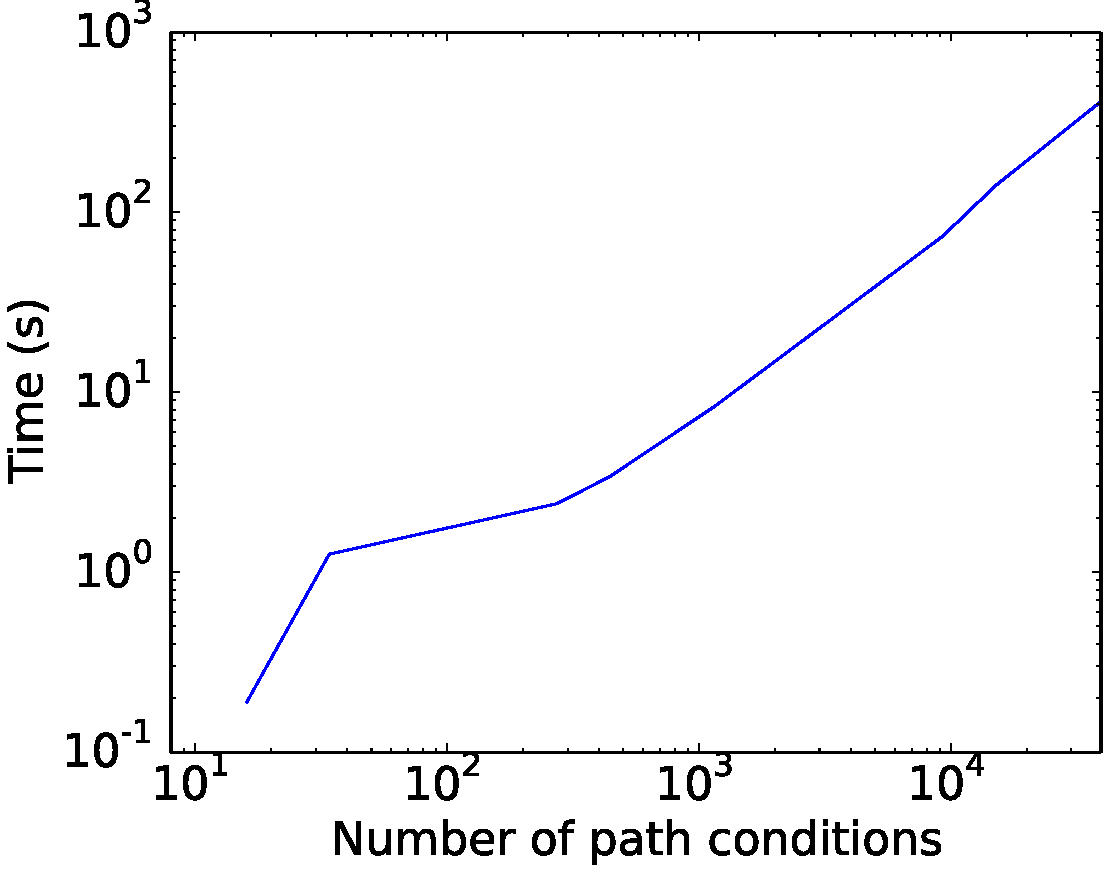
\includegraphics[width=0.35\textwidth]{./figures/results/pcs_vs_prop1.pdf}
	\caption{Time required to prove the property that holds on all path conditions}
	\label{fig:pcs_vs_prop1}
\end{figure}

\cref{fig:pcs_vs_prop1} shows the time in seconds required to prove the property that holds on all path conditions, as seen in the fifth column in \cref{tab:scalability_results}. Note that the time taken increases linearly with the number of path conditions to examine. This increase occurs as each property must be checked to ensure that the property will hold.

In contrast, the time required to disprove the property that does not hold is roughly constant. This can be seen in the sixth column in \cref{tab:scalability_results}, where this proof took 0.003 seconds regardless of the number of path conditions examined. This is due to the fact that, given the property does not hold, the proof algorithm can stop as soon as a counterexample is found. The very short time to disprove the property is due to the fact that path conditions are checked for the property sequentially, in the order they are produced. In our example, a counterexample can be found very early in the set of path conditions. Note that a more complex property that involves rules which would appear only much later in the generated set of path conditions would require a longer time to reach a counter-example.

Experiments were also undertaken to determine what effects the size of the property to be proved has on the running time of the algorithm. Preliminary results indicate that an increase of the property size results in a proportional increase in running time. This is to be expected, as the underlying graph matching algorithm has to match more elements to determine if the property holds or not.

% \levi{Do you want to keep this?}
% Finally, one last observation on the values in
% table~\ref{tab:scalability_results} is the fact that when rules without backward
% links are added to the transformation (the jumps from~7 to~10,~14 to~17 and~21
% to~24 rules) both the number of produced path conditions and the used memory
% increases around tenfold. Comparatively, when rules with backward links are
% added to the transformation (the jumps from ~3 to~7,~10 to~14 and 17 to~21
% rules) both the number of path conditions and the used memory only increases
% around five times. This is despite the fact that we increase rules with backward
% links by sets of 4 rules, whereas we increase rules without backward links by
% sets of 3 rules. The reason for this difference is the fact that, during
% symbolic execution construction, a rule with backward links may simply not be
% executable for a given path condition or can be merged with a previous path
% conditions. In both these cases no new path conditions are added to the symbolic
% execution. However, a rule without backward links necessarily generates twice
% the path conditions already generated by the symbolic execution algorithm as it
% may always be executed.
% 
% \levi{talk about better time optimizations here}It is however the case that, if
% no or few collapse operations are required for a path condition, the algorithm
% still attempts to collapse rules in this fashion. This may result in overhead as
% compared to merging all the rules and recursively collapsing. 

\subsection{Industrial Experimentation}
\label{sec:industrial_exp}

Aside from the experiments with the police station transformation we have
reported in the previous section, we have applied our technique in the context
of the NECSIS project.
The experiment regards a DSLTrans transformation that maps between subsets of a
proprietary metamodel from General Motors, describing legacy automotive configuration data, and
the AUTOSAR metamodel, an open platform shared by car manufacturers. This DSLTrans mapping transformation includes seven rules, distributed among three
layers. Further details of this experiment can be found in~\cite{gehan:13} and a complete description of the transformation can be found in~\cite{SelimWCD12}.

Our path condition generation approach generates a set of three path conditions for the transformation in approximately 0.8 seconds. This low number of path conditions is
due to the fact that several rules overlap, as explained in \cref{def:layer_transformation} of \cref{sec:formal_background}. Such overlapping causes the number of formed path conditions to be smaller than in the case where no overlaps occur, as certain combinations need not be considered due to rule dependency.

In~\cite{conf/gg/SelimLCDO14} we also describe the proof of nine properties (multiplicity invariants, security invariants and pattern contracts) that demonstrate several aspects of the correctness of this mapping transformation. The proof of these properties on all executions of a migration transformation is of interest to our industrial partners in order to ensure that the migration does not add extraneous elements or delete any needed information.

All properties were proved in around 0.02 seconds by our approach, and were expressed using a propositional logic extension to the property language that we present in this paper. Note that, despite the fact that not all aspects of the case study (overlapping rules, propositional logic extension) are considered theoretically in this manuscript, the obtained results are nonetheless very interesting in terms of the experimental scalability of our approach. In particular, we note that our verification approach performs orders of magnitude faster compared to an ATL-based verification tool that verified the same transformation~\cite{conf/gg/SelimLCDO14}.

\subsection{Discussion}

The experimental results of verifying the test Police Station transformation
portrayed in the graphs of \cref{fig:path_condition_building} show that,
as predicted by complexity \cref{eq:complexity}, both the path condition
construction time and the number of created path conditions grow exponentially
with the number of rules.
In \cref{fig:pcs_vs_prop1} we can also see that property proving time for
properties that hold increases linearly with the number of path conditions, as
was also theoretically predicted in \cref{sec:complexity}. Despite the exponential time
and space complexities of the path condition construction algorithms, our
experiments suggest that real-world sized model transformations can be tractable
by employing the optimizations described in \cref{sec:optimization}.
We also believe further optimization opportunities of our algorithms exist and that the number of rules handled by our approach can be driven higher.

The industrial case study presented in \cref{sec:industrial_exp} suggests
that validation of practical model transformations is not always very
computationally expensive. In fact, the properties we have proved in this
industrial case study are of practical use for our partners, yet required only fractions of seconds to prove.

From the differences in the examples we have presented in this section and from
our experience with building DSLTrans transformations we believe that the
complexity of verifying real-word model transformations can vary within a wide
range. The complexity of \cref{eq:complexity} provides us a referential that can
be used when evaluating the theoretical and operational complexities of
verifying further case study transformations. This complexity is influenced by several parameters that describe the shape of a model
transformation, and we believe the study of those parameters in further case studies is very
important. Refining \cref{eq:complexity} will provide better precision in our theoretical estimations and also direct our
optimization efforts by understanding what transformation parameters have the
highest impact on performance.

%  Refine the complexity formula to get better precision. Our problem
% is tractable using some implemention tricks. 
% 
% It's the same order of complexity
% for PC construction and property proof (despite disambiguation being done during
% property proof). The graphs show that we still have exponential curves that are
% flatter than expected due to optimizations. Future work will involve finding the
% more likely values for the parameters in our formula and thus optmize for them.
% This will provide guidance for optimization implementation and provide better
% definition of the expected vs real performance.
% 
% It does match our expectations, but is does not look bad.
% 
%  However, as can be seen in graph\levi{add graph with
% expected vs real number of path conditions and times}, our results are much
% better than predicted which suggests the problem is manageable when the number
% of rules is kept to a reasonable size and given our optimizations introduced in
% section~\ref{sec:optimizations}.




% The expected complexity of building the path
% conditions our experiment involving 21 rules as shown in
% table~\ref{table:results} can be calculated by instantiating the parameters of
% formula~\ref{eq:complexity} as $r=5$ (average number of rules per layer), $l=4$
% (number of layers), $e=2$ (average number of elements having the same type as
% elements in other rules of the same layer), $c=2$ (average pairs of rules per
% layer share common elements). We reach a final value of 5.308.416

% The performance results are promising, but
% further experiments with other transformations need to be done in order to
% assess the real performance of our approach. In fact, depending on the size of
% the rules in the considered model transformation, on rule distribution among
% layers, if those rules involve many backward links or not and whether many
% elements of the same type exist scattered by different rules or not (implying
% many collapse operation), we expect that the number of rules that can be tackled
% by our approach may vary substantially.\levi{need to finish this}
